\section{USB}

In order to configure the FPGA we load the configuration bit stream onto the board using a US cable
and USB micro receptor on the PCB. The signal is then passed along to
an \href{http://www.ftdichip.com/Support/Documents/DataSheets/ICs/DS_FT2232H.pdf}{FT2232H} IC
that translates the USB signal into JTAG data which it sends to the FPGA using the TCK, TDI, TDO and
TMS pins. The schematic for this is shown in Figure~\ref{fig:usb-ft2232}. The FT2232H IC
requires several power inputs: 3 VCORE input pins that require a 1.8V input voltage (this comes from
VREGOUT, which is a pin that outputs a 1.8V signal from an internal voltage regulator), 1 3.3V VREGIN
input (which serves as the input pin to drive the 1.8V regulated output), 4 3.3V VCCIO input pins,
and 23.3V inputs (VPLL and VPHY) that are filtered with an LC filter.

\paragraph{FIXME} I'm a bit confused as to the operation of the LC filter. It is implemented as a
ferrite bead with two parallel capacitors in parallel with the load. This feeds in from an LDO
regulator that in turn received its input from a buck converter operating at roughly 700kHz. The
frequency at which the ferrite bead is in its resistive state is around 100MHz, well above the
switching regulator noise. Maybe the filter is meant to filter out noise other than that from the
buck converter. For instance, it is possible that the LDO regulator used after the buck converter
(which has a PSRR near 0 around 500kHz and above) is sufficient for filtering the switching
noise. The Art of Electronics states that ferrite beads should be placed at different points
throughout the design to raise impedance at high frequencies. It is possible that this is the
functionality provided by these ferrite beads.  OSCI and OSCO are the oscillator input and output,
respectively. These must be connected to a 12MHz oscillator with a frequency tolerance less than
30ppm (ours is 10ppm). REF is a current reference that must be connected to a 12k$\Omega$ resistor to
ground. DM and DP are the USB data signal minus and plus lines, respectively. TEST should be
connected to ground. RESET\# (the \# indicates an active low pin) is connected to a pull-up resistor
to 3.3V so the reset is deasserted whenever the input voltage is at a sufficiently high and stable
level. PWREN\# is an output that is 0 during normal operation. We don't need it here so we leave it
floating. SUSPEND\# is similar to PWREN\#; it is low when the USB is in suspend mode. This is used as
an input to the FPGA. BDBUS0-3 are used for the JTAG interface to configure the FPGA. In order, they
are TCK, TDI, TDO and TMS.

\subsection{FT2232H}
\label{sec:ft2232h}

\paragraph{FIXME} The FT2232H device also communicates with the FPGA using a synchronous FIFO
interface as described
\href{http://www.ftdichip.com/Support/Documents/AppNotes/AN_130_FT2232H_Used_In_FT245\%20Synchronous\%20FIFO\%20Mode.pdf}{here}. This
seems to be the way that data is sent between the FPGA and the host computer although I'm not
clear how this works. In any event, it uses the ADBUS0-7 and ACBUS0-7 pins. The ADBUS pins
are bidirectional pins that serve as the FPGA side translation of the USB data. In other words,
they should allow the FPGA to read USB data from a host computer and send data back to that host
computer through a USB cable. The ACBUS lines seem to be used to signal reads/writes/etc. It also
seems to require the external EEPROM storage IC,
\href{http://ww1.microchip.com/downloads/en/DeviceDoc/20001749K.pdf}{93LC46B} although I'm not sure
why this interface requires additional, external memory.

\begin{figure}[h]
  \centering
  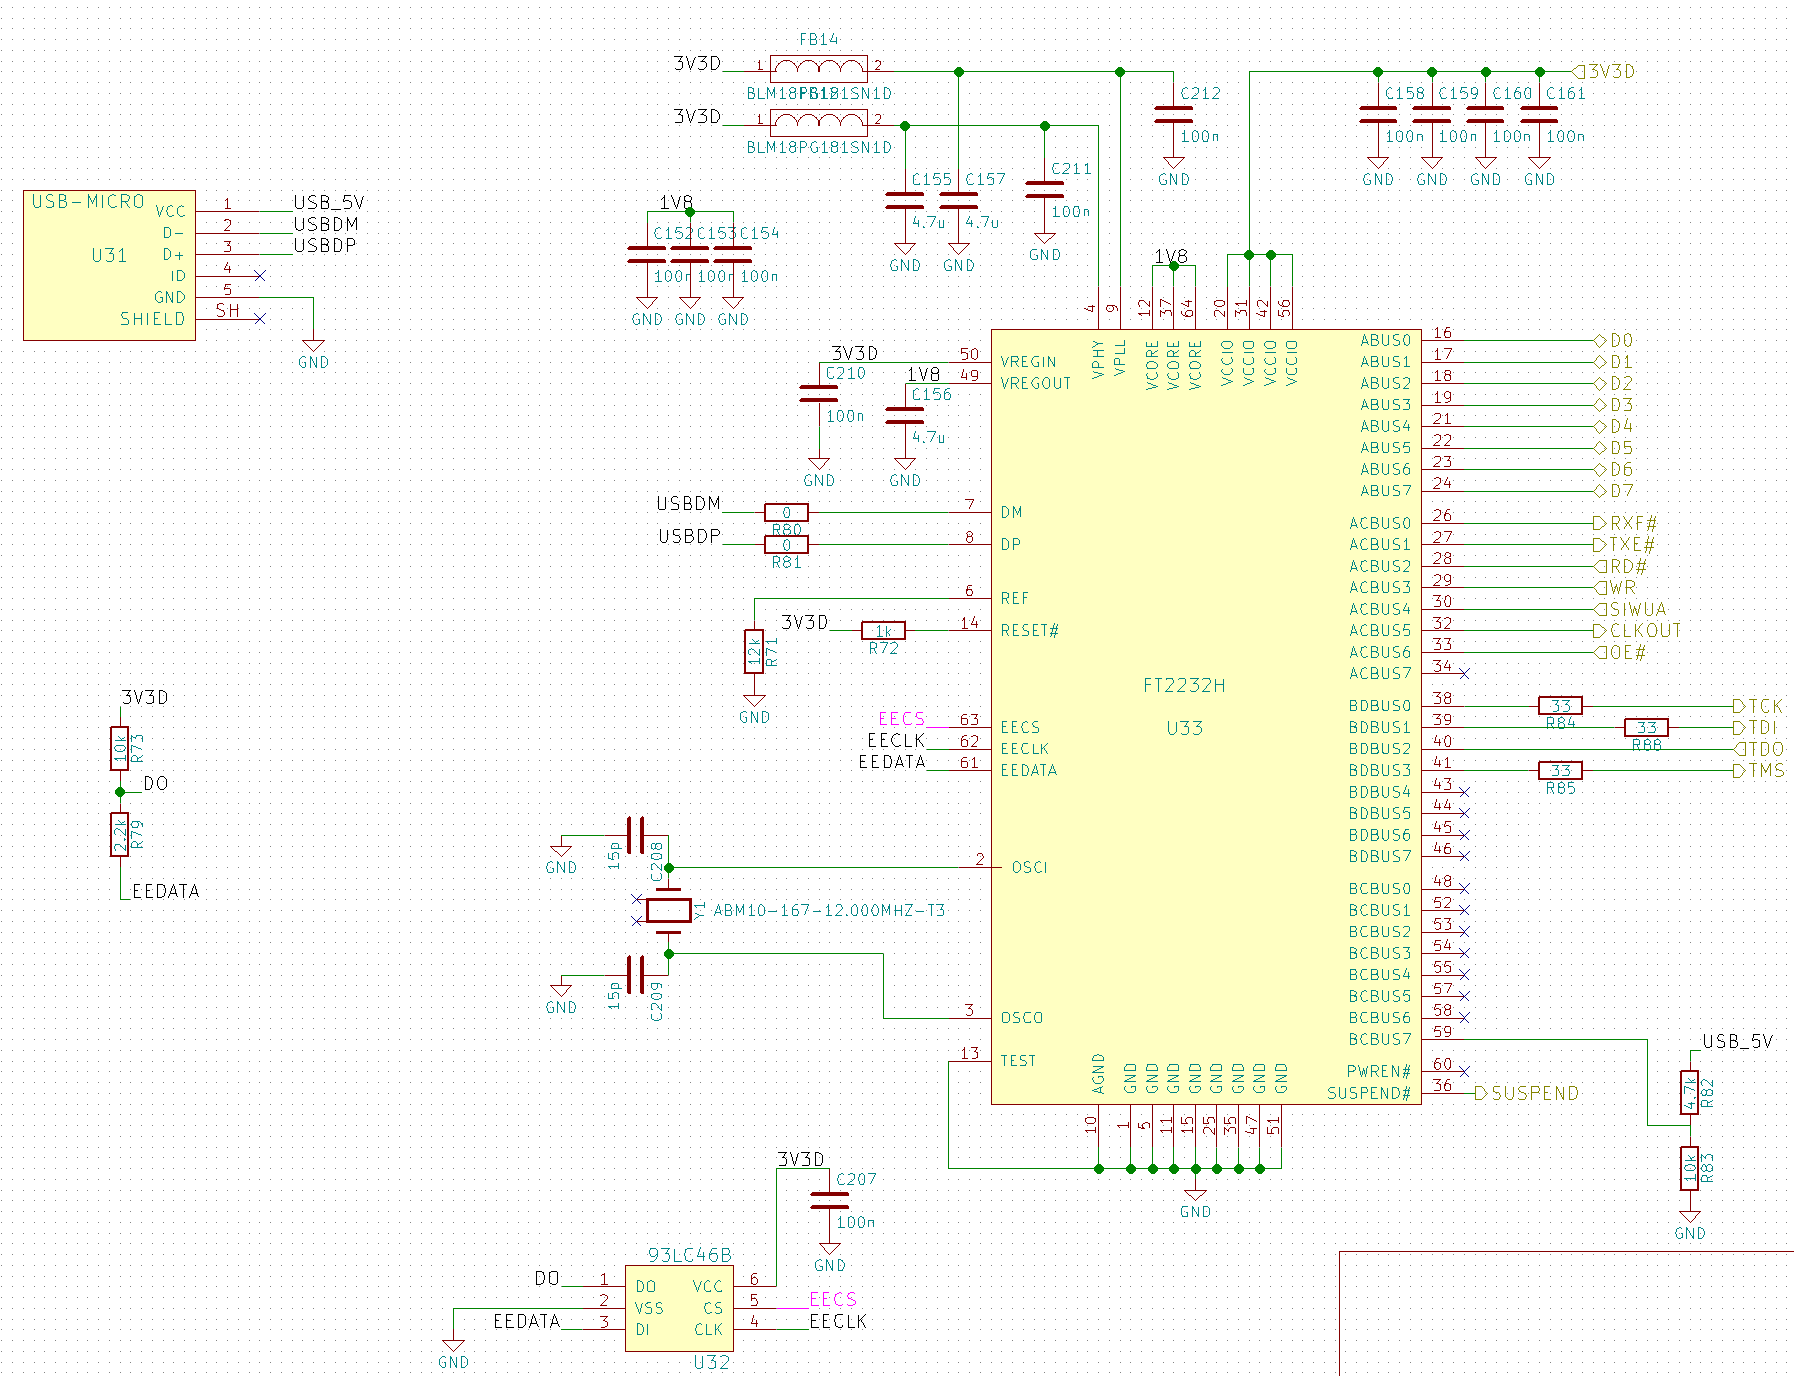
\includegraphics[width=\textwidth]{data/usb-ft2232.png}
  \caption{The configuration bit stream is loaded onto the FPGA using a USB-JTAG interface.}
  \label{fig:usb_ft2232}
\end{figure}

\subsection{93LC46B 1k EEPROM}
\label{sec:93lc46b}
